% !TEX encoding = UTF-8 Unicode
% -*- coding: UTF-8; -*-
% vim: set fenc=utf-8

\chapter{Abordagem para análise de rastros de proveniência}%
\label{chap:rastros-de-proveniencia}

% ilustrar com query SQL, tabela, grafo (img)

\section{Visão geral sobre a análise de rastros de proveniência}

 % definição, etc
 
\section{Tipos de rastros de proveniência}

% explicação + exemplo + complemento de uma (sub)seção anterior

\subsection{Físico}

\subsection{Lógico}

\subsection{Híbrido}

% \section{DfAnalyzer: Uma instanciação da arquitetura ARMFUL para análise dos rastros de proveniência}

\section{Query Processor}

O Query Processor foi implementado na linguagem de programação Java...

\perrotta{TODO: EXPAND ++ TODO: Mencionar o pré-processamento e as otimizações que fiz}

\section{Algoritmos utilizados}%
\label{sec:algoritmos-utilizados}

Nessa seção serão abordados os principais algoritmos e funções utilizadas no Query Processor. Funções auxiliares referenciadas pelos mesmos estão definidas no \autoref{app:funcoes-auxiliares}. A notação utilizada é de pseudocódigo, e as definições dos algoritmos e nomes das variáveis utilizados foram ligeiramente alterados e simplificados em relação à implementação original, visando uma melhor clarificação e apresentação do código.

\perrotta{REVIEW: mencionar algo a mais sobre a notação?}

\subsection{Detecção das últimas transformações de dados}

O \autoref{lst:algorithm-last-transformations} demonstra como obter as \textbf{últimas transformações de dados} \texttt{transformations} de um fluxo de dados \( D \), isto é, as transformações de dados \(dt\) as quais não possuem nenhuma outra transformação de saída após as mesmas. A ideia do algoritmo é bastante simples: basta checar todas as dependências de dados \( \phi \) --- do conjunto de dependência de dados do fluxo de dados \( D.\Phi \) --- cujo \( dt_{\textrm{next}} \) é nulo, e tomar o \( dt_{\textrm{previous}} \) das mesmas.

% https://tex.stackexchange.com/questions/73231/avoid-page-breaks-in-lstlistings
\begin{minipage}[c]{0.95\textwidth}
\begin{lstlisting}[language=pseudocode,label={lst:algorithm-last-transformations},caption={[Detecção das últimas transformações de dados]Detecção das útimas transformações de dados em uma especificação de fluxo de dados.}]
function getLastTransformations(%\(D\)%):
    transformations %\leftarrow% {}
    for each %\phi% %\in% %\(D.\Phi\)% do:
        if %$\phi.dt_{\texttt{next}} = \varnothing$% then:
            transformations %\leftarrow% transformations + 
        end if
    end do
    return transformations
end function
\end{lstlisting}
\end{minipage}

A complexidade de tempo do algoritmo é linear da ordem de \( O(\#(D.\Phi)) \), isto é, proporcional ao número de dependências de dados do fluxo de dados \( D \), e as transformações retornadas pelo algoritmo são armazenadas em uma simples lista encadeada, já que não é necessário acesso aleatório a essa estrutura de dados. Entretanto, na prática, com o objetivo de amortizar um pouco a complexidade, esse algoritmo é aplicado \textit{on-the-fly}, no momento em que o fluxo de dados é construído e instanciado no QP (c.f. \autoref{subsec:preprocessamento}).

\subsection{Detecção das trilhas de transformações}%
\label{subsec:deteccao-das-trilhas-de-transformacoes}

O \autoref{lst:algorithm-transformation-tracks} demonstra como obter as \textbf{trilhas de transformações} \texttt{dtTracks} de um fluxo de dados \( D \). As trilhas são uma maneira natural de separar e agrupar transformações de dados em vários subconjuntos, definidos e limitados através de separações (do inglês, \textit{splits}) em \( D \). Tais separações existem no grafo do fluxo de dados em interseções de transformações que possuem mais de uma transformação de entrada ou de saída (\textit{i.e.}, grau do vértice maior do que 1). Por exemplo, na \autoref{fig:transformation-tracks}, podemos visualizar um exemplo de divisão e agrupamento de transformações de dados em trilhas.

\begin{figure}[htb]
    \centering
    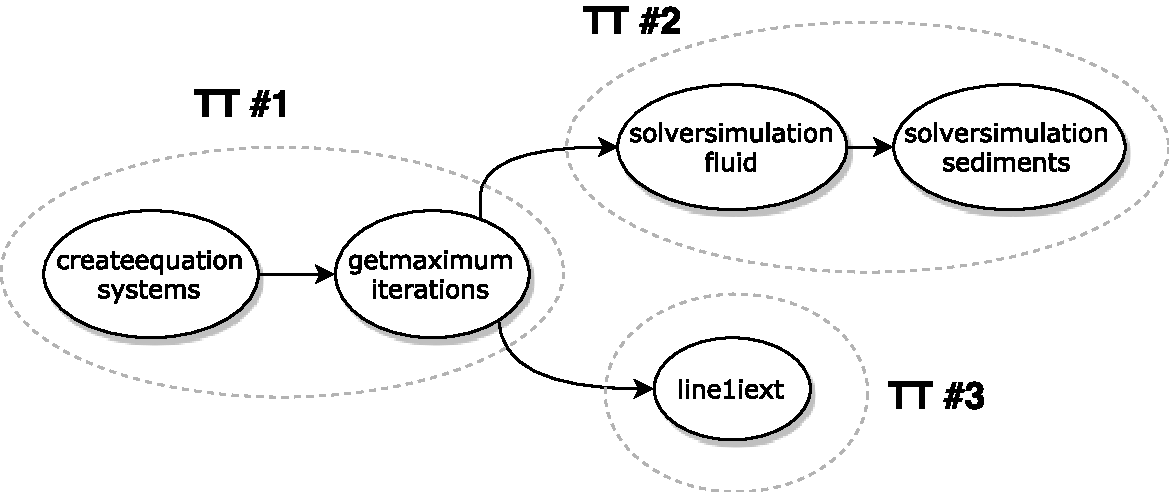
\includegraphics[width=\textwidth]{img/transformation-tracks}
    \caption[Exemplo de detecção das trilhas de transformações.]{Exemplo de detecção das trilhas de transformações de um fluxo de dados. Na figura existem três trilhas de transformações (\textsc{TT}).}%
    \label{fig:transformation-tracks}
\end{figure}

O algoritmo começa com as últimas transformações \texttt{lastDts} de \( D \) (encontradas no \autoref{lst:algorithm-last-transformations}), e caminha em direção às primeiras transformações de \( D \), utilizando uma estrutura de dados \texttt{queue} do tipo fila (FIFO - \textit{First In First Out}) como armazenamento temporário das próximas transformações de dados a serem analisadas. A ideia principal é realizar a detecção do fim --- e, consequentemente, também do início --- de cada trilha de transformação \texttt{dtTrack}, que pode acontecer em várias situações: \textit{e.g.}, sempre que o grau de saída do vértide de uma transformação for maior do que 1, indicando que a transformação em questão possui várias transformações de saída.

\begin{minipage}[c]{0.95\textwidth}
\begin{lstlisting}[language=pseudocode,label={lst:algorithm-transformation-tracks},caption={[Detecção das trilhas de transformações]Detecção do rastro do fluxo de dados no nível de trilhas de transformações.}]
function getTransformationTracks(%\(D\)%):
    dtTracks %\leftarrow% {}
    lastDts %\leftarrow% getLastTransformations(%\(D\)%)%~\quad%#%~\autoref{lst:algorithm-last-transformations}%
    queue %\leftarrow% {}%~\quad%#%~%FIFO (First In First Out)
    queue.enqueue(lastDts)
    while queue is not empty do:
        dt %\leftarrow% queue.dequeue()
        nextDts %\leftarrow% getNextTransformations(%\(D\)%, dt)
        if dt %\in% lastDts
           or hasManyOutputDatasets(%\(D\)%, dt)
           or hasManyNextTransformations(%\( D \)%, dt)
           or anyTransformationHasManyInputDatasets(%\(D\)%, nextDts)
           then:
            dtTrack %\leftarrow% {dt}
            dtTracks %\leftarrow% dtTracks + {dtTrack}
        else then:
            dtTrack %\leftarrow% getTransformationTrack(dtTracks, nextDts[0])
            dtTrack %\leftarrow% dtTrack + {dt}
        end if
        previousDts %\leftarrow% getPreviousTransformations(%\(D\)%, dt)
        queue.enqueue(previousDts)
    end do
    return dtTracks
end function
\end{lstlisting}
\end{minipage}

A complexidade de tempo do algoritmo é linear da ordem de \( O(\#(D.\Phi)) \), como no \autoref{lst:algorithm-last-transformations}. As trilhas de transformações \texttt{dtTracks} são armazenadas em listas encadeadas de transformações --- acesso aleatório não é necessário, porém convém armazená-las na mesma ordem em que foram encontradas.

\subsection{Detecção das trilhas de conjuntos de dados}

O \autoref{lst:algorithm-dataset-tracks} tem como função obter as \textbf{trilhas de conjuntos de dados} \texttt{dsTracks} de um fluxo de dados \( D \). O conceito de trilha de conjuntos de dados é análogo e baseado no de trilha de transformações de dados, mencionado na \autoref{subsec:deteccao-das-trilhas-de-transformacoes}: é uma forma de dividir e agrupar conjuntos de dados em diversos subconjuntos.

O algoritmo funciona com base no \autoref{lst:algorithm-transformation-tracks}: uma vez tomadas as trilhas de transformações de dados \texttt{dtTracks}, é simples obter cada uma das trilhas de conjuntos de dados \texttt{dsTrack} a partir de cada \texttt{dtTrack}. Para isso, basta tomar a união de todos os conjuntos de dados adjacentes (\textit{i.e.} anteriores e posteriores) a todas as transformações de dados de \texttt{dtTrack}.

\begin{minipage}[c]{0.95\textwidth}
\begin{lstlisting}[language=pseudocode,label={lst:algorithm-dataset-tracks},caption={[Detecção das trilhas de conjuntos de dados]Detecção do rastro do fluxo de dados no nível de trilhas de conjuntos de dados.}]
function getDatasetTracks(%\(D\)%):
    dsTracks %\leftarrow% {}
    dtTracks %\leftarrow% getTransformationTracks(D)%~\quad%#%~\autoref{lst:algorithm-transformation-tracks}%
    for each dtTrack %\in% dtTracks do:
        dsTrack %\leftarrow% {}
        for each dt %\in% dtTrack do:
            if dsTrack is empty then:
                dsTrack %\leftarrow% dsTrack + {getNextDatasets(%\(D\)%, dt)}
            end if
            dsTrack %\leftarrow% dsTrack + {getPreviousDatasets(%\(D\)%, dt)}
        end do
        dsTracks %\leftarrow% dsTracks + {dsTrack}
    end do
    return dsTracks
end function
\end{lstlisting}
\end{minipage}

A complexidade de tempo do algoritmo é a mesma do algoritmo do \autoref{lst:algorithm-transformation-tracks}: linear da ordem de \( O(\#(D.\Phi)) \), e as trilhas de conjuntos de dados \texttt{dsTracks} são também armazenadas em listas encadeadas de conjuntos de dados.

\subsection{Obtenção de múltiplos mapeamentos de atributos entre dois conjuntos de dados}

O \autoref{lst:algorithm-attribute-mappings} demonstra como obter \textbf{múltiplos mapeamentos de atributos}...

\perrotta{TODO: introduction with caption repeating + algorithm explanation. Reiterate the definition of mapeamentos de atributos (seção 2, das definições).}

\begin{minipage}[c]{0.95\textwidth}
\begin{lstlisting}[language=pseudocode,label={lst:algorithm-attribute-mappings},caption={[Obtenção de múltiplos mapeamentos de atributos]Obtenção de múltiplos mapeamentos de atributos entre dois conjuntos de dados adjacentes.}]
function getAttributesMapping(dt,%\(ds_{\textrm{input}}\)%,%\(ds_{\textrm{output}}\)%,type)
   attrs %\leftarrow% {}
   if type = physical then:
       attrs %\leftarrow% attrs + {t.getInstanceAttribute()}
   else:
       for each inAttr %\in% %\(ds_{\textrm{input}}\).A% do:
           for each outAttr %\in% %\(ds_{\textrm{output}}\).A% do:
               if inAttr.name = outAttr.name
                  and inAttr.type = outAttr.type then:
                   attrs %\leftarrow% attrs + {inAttr}
               end if
           end do
       end do
   end if
   return attributesMapping(attrs,dt,%\(ds_{\textrm{input}}\)%,%\(ds_{\textrm{output}}\)%)
end function
\end{lstlisting}
\end{minipage}

\perrotta{TODO: complexity and data structures}

\subsection{Obtenção dos caminhos entre dois conjuntos de dados}

A função \texttt{findPaths} do \autoref{lst:algorithm-find-paths} inicializa a estrutura de estados \texttt{state}, necessária para a chamada da função de busca em profundidade \abbrev{DFS}{Depth-first Search (Busca em profundidade)} \texttt{depthFirstSearch} (DFS) do \autoref{lst:algorithm-dfs}. Essas duas funções atuam em conjunto com um objetivo em comum: \textbf{obter todos os caminhos entre dois conjuntos de dados} \texttt{dsOrigin} e \texttt{dsDestination} do fluxo de dados \(D\).
Nesse contexto, um caminho é definido como uma lista ordenada de conjuntos de dados, cujo primeiro elemento é \texttt{dsOrigin}, e cujo último elemento é \texttt{dsDestination}.

Como podem existir potencialmente vários caminhos entre esse par de conjuntos de dados, a função \texttt{findPaths} possui dois argumentos adicionais que atuam como filtros:

\begin{itemize}
    \item \texttt{dsIncludes} --- uma coleção de conjuntos de dados: todos eles devem estar presentes no caminho para que tal caminho seja retornado pela função \texttt{findPaths};
    \item \texttt{dsExcludes} --- o oposto de \texttt{dsIncludes}: nenhum dos caminhos que fazem parte da coleção \texttt{dsExcludes} pode estar presente nos caminhos retornados por \texttt{findPaths}.
\end{itemize}

\begin{minipage}[c]{0.95\textwidth}
\begin{lstlisting}[language=pseudocode,label={lst:algorithm-find-paths},caption={[Obtenção dos caminhos entre dois conjuntos de dados.]Obtenção de todos os caminhos entre dois conjuntos de dados, inicializando a \textsc{DFS} com um estado inicial apropriado.}]
function findPaths(D,dsOrigin,dsDestination,dsIncludes,dsExcludes)
    state %\leftarrow% {}
    state.visited %\leftarrow% {dsOrigin}
    state.paths %\leftarrow% {}
    state.dsOrigin = dsOrigin
    state.dsDestination = dsDestination
    state.dsIncludes = dsIncludes
    state.dsExcludes = dsExcludes
    depthFirstSearch(D, state)%~\quad%#%~\autoref{lst:algorithm-dfs}%
    return state.paths
end function
\end{lstlisting}
\end{minipage}

A função \texttt{depthFirstSearch}

\perrotta{TODO: algorithm explanation + complexity + data structures.}

\begin{minipage}[c]{0.95\textwidth}
\begin{lstlisting}[language=pseudocode,label={lst:algorithm-dfs},caption={[Busca em Profundidade (DFS) dos caminhos]Depth First Search (DFS): busca em profundidade de todos os caminhos entre dois conjuntos de dados.}]
function depthFirstSearch(D,state)
    nodes %\leftarrow% getNextDatasets(D,state.visited.getLast())
    for each node %\in% nodes do:
        # Pular nós que já foram visitados.
        if node %\in% state.visited then:
            continue
        end if
        # Checar se está no fim da DFS.
        if node = state.dsDestination then:
            state.visited %\leftarrow% state.visited + {node}
            path %\leftarrow% new Path(state.visited)
            if state.dsIncludes %\in% path and state.dsExcludes%~%%\not\in%%~%path then:
                state.paths %\leftarrow% state.paths + {path}
            end if
            state.visited.pop()
            break
        end if
    end do
    for node %\in% nodes do:
        if node %\in% state.visited or node = state.dsDestination then:
            continue
        end if
        state.visited %\leftarrow% state.visited + {node}
        depthFirstSearch(state)
        state.visited.pop()
    end do
end function
\end{lstlisting}
\end{minipage}

\subsection{Geração da consulta em SQL}

\perrotta{TODO: everything. Autoref code label, Bold title, Introduction with caption repeating + algorithm explanation. Later: Complexity, data structures.}

\begin{minipage}[c]{0.95\textwidth}
\begin{lstlisting}[language=pseudocode,label={lst:algorithm-generate-sql-query},caption={[Geração da consulta em SQL]Geração da consulta na linguagem SQL a partir das especificações do usuário.}]
function generateSqlQuery(D,dsOrigins,dsDestinations,dsIncludes, dsExcludes,type,projections,selections)
    selectClause %\leftarrow% {}
    fromClause   %\leftarrow% {}
    whereClause  %\leftarrow% {}
    for each projection %\in% projections do:
        selectClause %\leftarrow% selectClause + {projection}
    end do
    for each selection %\in% selections do:
        whereClause %\leftarrow% whereClause + {selection}
    end do
    for each dsOrigin %\in% dsOrigins do:
        for each dsDestination %\in% dsDestinations do:
            paths %\leftarrow% findPaths(dsOrigin, dsDestination, dsIncludes, dsExcludes)%~\quad%#%~\autoref{lst:algorithm-find-paths}%
            for each path %\in% paths do:
                for each ds %\in% path do:
                    fromClause %\leftarrow% fromClause + {ds}
                end do                
                for (i %\leftarrow% 1; i < path.size(); i %\leftarrow% i + 1) do:
                    prevDs %\leftarrow% path[i - 1]
                    nextDs %\leftarrow% path[i]
                    attrMapping %\leftarrow% getAttributesMapping(D.getTransformation(prevDs, nextDs), prevDs, nextDs, type)%~\quad%#%~\autoref{lst:algorithm-attribute-mappings}%
                    for each attr %\in% attrMapping do:
                        whereClause.addSelection(prevDs.attr, "=", nextDs.attr)
                        if projections is empty then:
                            selectClause %\leftarrow% selectClause + {prevDs.attr, rightDs.attr}
                        end if
                    end do
                end do
            end do
        end do
    end do
    sqlQuery %\leftarrow% new SqlQuery(selectClause, fromClause, whereClause)
    return sqlQuery
end function
\end{lstlisting}
\end{minipage}

\subsection{Pré-processamento}%
\label{subsec:preprocessamento}

\section{Um exemplo}

\perrotta{como rodar o algoritmo -- explicar a assinatura da função principal e exemplos de uso (chamadas)}